\subsection{Tuning of VNS}

\begin{figure}[!h]
    \centering
    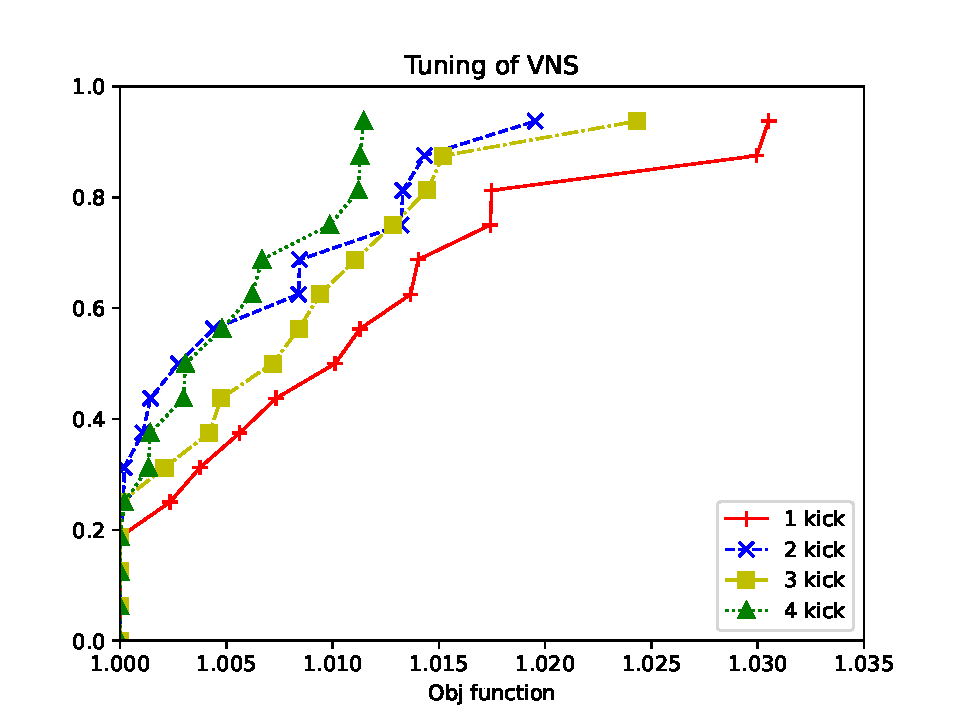
\includegraphics[width=\textwidth]{images/vns.pdf}
    \caption{VNS Tuning of number of kicks}
    \label{fig:vns}
\end{figure}

The VNS algorithm can vary its efficiency depending on how many kicks it computes at each iteration.

After some tests we noticed that the size of the instance didn't really affected the decision of how many kicks to make, so we made a comparison using the same number of kicks for each instance, disregarding its actual size, see Figure \ref{fig:vns}.

